\cleardoublepage

\section{绪论}

\subsection{研究的背景与意义}
\par 随着现代医学的不断发展和医疗技术水平的不断提高,人类在面对疾病时也有了越来越多的手段以解决越来越多的疑难杂症,全球人类的平均寿命也在不断延长,然而,许多常见的癌症却不在此列。宫颈癌是女性最常见的癌症之一,严重威胁着全球女性的生命安全和身体健康。2018年,全球约有57万女性确诊宫颈癌,约31.1万女性因宫颈癌逝世。然而,宫颈癌的发病过程是缓慢增长的,从癌前病变到病发的时间通常是5年或更长,这为通过早期科学有效的检测手段发现和适当治疗降低宫颈癌的发病率和死亡率提供了机会。全世界大约七成的宫颈癌发生在发展中国家\cite{wild2014world},在发达国家中,因为宫颈抹片筛查以及其他检测方法的普及,宫颈癌的发病率和致死率大大降低\cite{canavan2000cervical}。这也说明,定期进行科学的宫颈癌筛查是十分必要的。
\par 宫颈癌筛查主要由“细胞学-阴道镜-组织学”三阶梯诊断程序组成,其中,作为第一道检测手段的细胞学筛查的主要作用是通过较低的成本和较快的检测速度实现大量的、普遍的筛查,一般来说,医生会先通过细胞学检测手段对患者进行诊断,如果没有发现异常的病变情况,患者就不再需要进行后续的检测了。因此,细胞学检测手段除了应当注重检测成本与检测速度以外,还应提高对病变细胞或组织的敏感程度,应当尽量能够检测出所有的病变情况。而由于细胞学检测只是第一道检测手段,阴道镜与组织学的检测手段可以更轻易地取得更为精确的检测结果,由此,细胞学检查中对检测结果的准确性要求相对会低一点。
\par 在临床上,细胞学检查的主要手段就是Thinprep cytologic test检查也即液基薄层细胞检测,简称TCT检查。在TCT检查过程中,医生需要使用专门的宫颈刷采集子宫颈脱落的细胞样本,再将细胞样本漂洗后转移到保存液瓶中,使用全自动细胞检测仪将细胞样本混匀、过滤,最后将细胞帖附到玻片上。医生将玻片染色固定后就可以使用显微镜观察细胞样本并做出诊断。
\par 这一过程通常需要医生通过显微镜在整个玻片上、上亿个细胞中寻找病变或疑似病变的细胞,最后根据全片中病变细胞的状况给出诊断。通常情况下,整个TCT样本的片子含有几亿甚至几十亿像素,十分巨大;玻片上也有上亿细胞,数目非常多。可想而知,全人工的阅片过程十分耗时费力,需要非常大的工作量。因此,我们亟需计算机的辅助手段来帮助医生完成TCT检查的阅片过程并进一步提升诊断的准确性。利用计算机辅助医生进行TCT检查既可以减少医生的工作量,又可以为TCT诊断引入一个相对客观的诊断结果,这对于医生和患者了解患者的病情以及开展后续的治疗工作等都是十分重要的。

\subsection{计算机辅助TCT检查面临的问题}
\label{sec:计算机辅助检查面临的问题}
\par 目前,已有许多目标检测方向和宫颈病变细胞检测方向的工作可以实现利用计算机辅助医生进行TCT检查的阅片工作的目的,然而,现有的宫颈病变细胞检测方法往往直接使用自然图像领域的目标检测方法,忽视了TCT检查图片的特点和其特有的问题,在检测性能上自然差强人意。也有部分研究针对这些问题做出了部分优化,例如,针对难以区分的类别加入了额外的分类器、使用了标签平滑等技术,其检测性能相较于自然图像领域的目标检测方法有所提升,但依然存在单细胞与细胞簇标注框形态差异大、TCT检查图片放大倍率不统一等问题,主要问题如下:

\subsubsection{单细胞与细胞簇的形态差异}
\label{par:单细胞与细胞簇的形态差异}
\par 医生在标注病变细胞框的时候,如果病变细胞是单个存在的、周围没有其他细胞的状态,那么医生会给该细胞单独标注一个框。但是,如果病变细胞聚集在一起形成了一个很大的细胞簇,那么病变细胞之间的界限会变得十分糢糊,只能选择标注一个很大的框将整个细胞簇框住。这就导致了同一种类标签的标注框有着两种不同的含义——既可以是单个的病变细胞,也可以是一整个病变细胞簇,而二者在形态上有着巨大的差异。
\par 例如,由于不论是病变细胞还是正常细胞细胞核往往在形态上处在整个细胞中心的位置,那么单个细胞对应的框的中心一般来说就是这个细胞的细胞核,因此从该处往往可以获得细胞核的形态特征。换句话说,如果网络发现了细胞核的形态特征,就可以将该点作为检测框的中心的进行预测。但是,如果框中的是一个大的细胞簇那么其中心就不再是明显的细胞核的特征了。而细胞核的形态特征又是判断病变与否已经病变种类的相当关键的特征,这就导致网络的学习过程中可能遇到难以学习的特征形态。与此类似的,单个细胞框的周围会是细胞质边界的特征,这也是判断病变细胞的一个重要特征,但是细胞簇的边缘是多个细胞聚集在一起时组成的形状,因为细胞是经过混匀的,这一形态信息完全由混匀过程决定可以认为是随机的,这对判断细胞的病变程度毫无意义。
\par 此外,单个细胞与细胞簇的界限并没有那么明显。例如,医生在标注框的时候,会遇到两三个细胞挨在一起的情况,这种情况下可以说为每个细胞单独标注框和将这两三个细胞视作一个细胞簇只标注一个框都是合理的。但这就给网络的学习带来了很大的难度——网络不仅要学会如何判断病变细胞,还需要学会制作训练用数据集的医生对于上述情况的偏好情况。而事实上,由于数据的标注由不止一位医生完成,往往每位医生对都上述情况会有不同的偏好,因此,网络可能根本无法学习到这一规律。这一问题严重地阻碍了网络的学习过程,然而,在实践中,我们往往并不关注病变细胞是有单独的框还是由一个框标注出来的,我们更关心病变细胞的召回率和病变等级判定的准确率。
\begin{figure}[h]
    \centering
    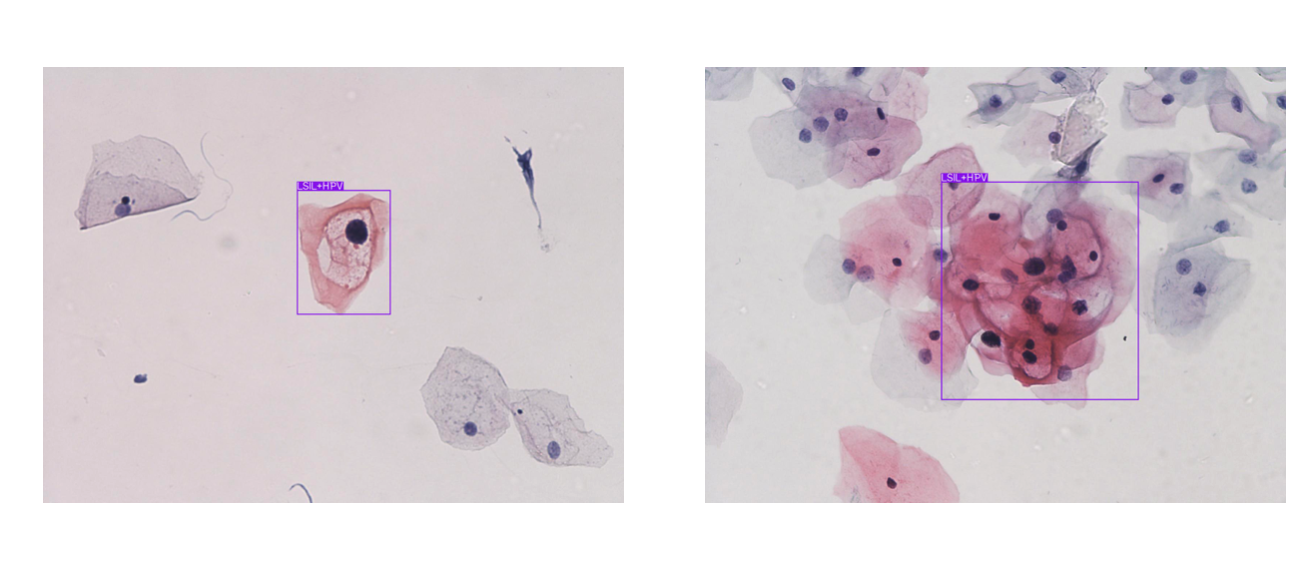
\includegraphics[width=0.5\paperwidth]{TCT/single_multi.png}
    \caption{单个病变细胞与病变细胞簇形态差异比较,左图为单个病变细胞,右图为许多病变细胞形成的细胞簇,两图中的病变细胞均为统一病变等级,但是由于细胞数目不同而具有完全不同的形态特征}
    \label{论文形态差异}
\end{figure}
\subsubsection{放大倍率不一致}
\par TCT检查的图片都是经过显微镜放大的,所以图片中细胞的绝对大小并没有实际的意义,甚至这一大小的变换还会为网络的学习带来阻碍。例如,涂片中可能出现一种叫做炎细胞的正常细胞,它相比于一般细胞会小得多,医生在做诊断时可以自然地忽略它,但是它的形态特征在放大之后与最高等级的病变细胞——鳞癌细胞的形态特征十分相近。他们的区别只是炎细胞相较与正常细胞非常小,而鳞癌细胞具有正常细胞的大小尺度。现有的深度学习方法主要通过FPN来生成各种尺度的图像金字塔来处理这种尺度变换的问题,但是,这种方法更适合用来检测尺度大小不确定的目标,对于形态特征相近只有尺度不同的目标,这种方式反而会影响网络的训练。
\begin{figure}[h]
    \centering
    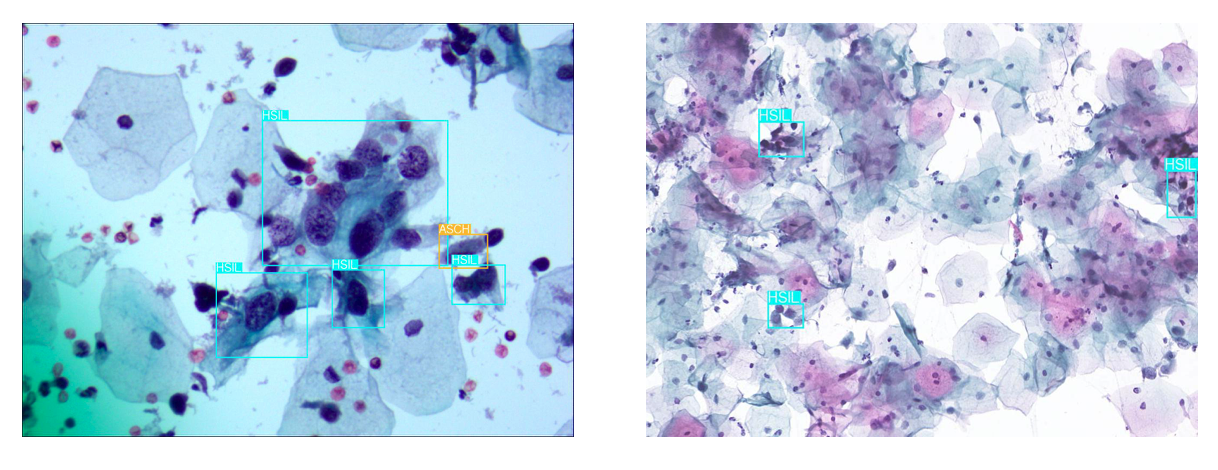
\includegraphics[width=0.5\paperwidth]{TCT/scale.png}
    \caption{不同图片之间放大倍率有着较大的差距,左图中的正常细胞大小相较右图中大得多,而实际上正常细胞的大小应当是一致的,所以左图放大倍率应当比右图高很多}
    \label{论文倍率差异}
\end{figure}

\subsection{论文主要研究内容}
\par 本文提出了一个全新的网络结构,使用了任务分解和细胞对比两大机制来完成宫颈病变细胞检测的任务。其中,针对上述单细胞与细胞簇的形态差异的问题,我们使用任务分解的方法,使用模型的不同模块分别捕捉两类目标的特征,并最终做出检测。针对TCT检查图片放大倍率不一致的问题,本文使用了细胞对比的方法,利用图片中的正常细胞的形态、尺寸特征增强了模型对于病变细胞类别的区分能力。这两大方法极大地增强了模型对于宫颈病变细胞检测任务的处理能力,有效地提升了模型的检测性能。

\subsubsection{任务分解}
\par 我们认为对于每个病变细胞的图像除去其病变类别以外,还应当分为单细胞或细胞簇两类,例如,对于某个病变细胞类别HSIL,应当分为HSIL-Single和HSIL-Multi两个类别,其中,HSIL-Single指的是标注框中只含有一个细胞的HSIL病变细胞标注框,而HSIL-Multi指的是含有两个及以上细胞的HSIL病变细胞标注框。然后,我们会使用不同的网络模块分别检测这两种类别,再将这两种类别的结果直接合并起来当作目标区域提案送入最终的检测头中进而取得最终的检测结果。

\subsubsection{细胞对比}
\par 在临床上,医生对检查结果做出诊断时也会面临放大倍率不统一的问题,医生在诊断时往往通过先在片子中寻找正常细胞,再以正常细胞的尺寸大小判断其他细胞病变与否以及病变种类的方法解决改问题。因此,我们在我们的模型中加入了细胞对比模块以模仿该过程。首先,我们的模型在检测异常细胞之前会先检测图片中的正常细胞并提取出正常细胞的特征,然后再使用正常细胞的特征与检测到的异常细胞的特征计算一个差分特征作为正常细胞与异常细胞对比的结果。我们还使用了一个专门设计的关系特征模块计算异常细胞与异常细胞之前的关系特征,最后,我们会综合这几个特征用于最后的异常细胞检测过程。

\subsection{本文的组织结构}
\par 本文共分为五章,各章节的主要内容和结构安排如下:
\par 第一章:绪论。本章主要介绍了研究的背景与意义、使用计算机辅助医生进行TCT检查时主要面临的问题以及本文的主要研究内容。本章首先介绍了宫颈癌与其筛查手段——TCT检查,之后讲述了医生在TCT检查过程中会遇到的问题,以及使用计算机辅助医生进行TCT检查会遇到的问题,并由此提出本文的主要创新点和研究内容。
\par 第二章:国内外研究现状。本章主要介绍了国内外利用计算机辅助医生进行宫颈病变细胞检查的研究工作,主要分为病变细胞的分类与分割和病变细胞的检测两个部分。本章介绍病变细胞的分类、检测与分割任务之后详细地介绍了国内外在宫颈病变细胞检测领域的相关工作情况。
\par 第三章:方法。本章主要介绍了我们模型的主要设计思路和设计细节,包含模型整体结构、任务分解和细胞对比两大机制以及使用半监督学习生成伪标签的介绍。本章首先整体描述了我们使用的网络结构,之后分别介绍了任务分解和细胞对比两大方法的运作方式和实现细节,最后介绍了我们使用半监督学习的方法为正常细胞生成伪标签从而使模型可以正常捕捉到正常细胞特征的过程。
\par 第四章:实验与结果。本章主要介绍了本文所设计的实验所使用的数据集、实验环境、实现细节、评价指标以及具体消融实验和对比实验的结果及分析。本章首先介绍了本文实验使用的数据集的主要状况。其次描述了我们使用的数据预处理手段和训练过程中的实现细节,之后介绍了我们使用的评价指标mAP,最后是我们设计的消融实验和对比实验的结果及其分析。
\par 第五章:总结与展望。本章主要总结了全文的主要内容并对后续可能的研究做出展望。本章首先对全文做出简要总结,然后列出了本文工作所具有的创新点,最后对本文研究内容后续可能的研究方法做了展望。

\clearpage

\section{国内外研究现状}
\label{sec:国内外研究现状}
\par 目前国内外通过计算机辅助医生进行宫颈TCT检测的方法主要分为病变细胞分类、病变细胞检测、病变部位分割三个部分。
\par 病变细胞分类主要是指仅给出输入视野中细胞的综合病变等级,一般会根据病变细胞的状况评定为在视野中出现的最高病变等级或者次高级。

\begin{figure}[h]
    \centering
    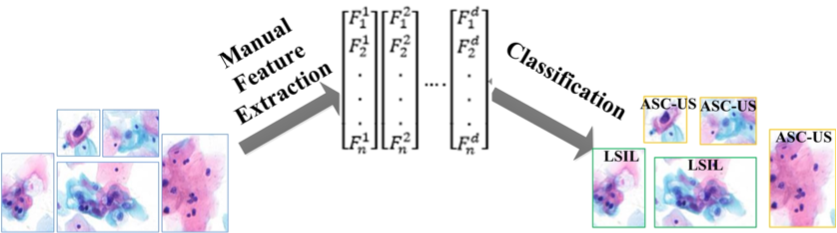
\includegraphics[width=0.5\paperwidth]{TCT/分类样例.png}
    \caption{病变细胞分类样例图片,输入图片经过提取特征等处理后由计算机判断图片所属的病变等级}
    \label{pic:分类样例}
\end{figure}
\par 病变细胞检测则是要求以矩形框的方式标注出视野内的病变细胞并给出病变等级,相较病变细胞分类任务而言,评定整个视野的综合病变等级的任务由医生完成。在病变细胞检测的任务中,计算机应当标注出所有病变细胞的位置并给每个病变细胞评定病变等级。

\begin{figure}[h]
    \centering
    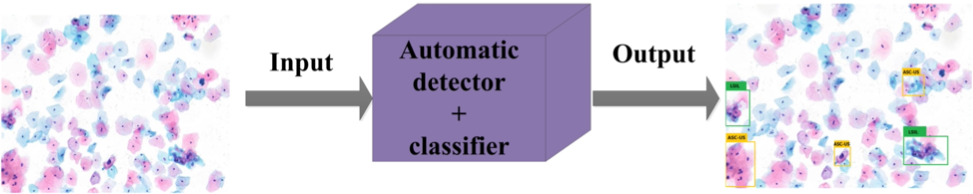
\includegraphics[width=0.5\paperwidth]{TCT/检测样例.png}
    \caption{病变细胞检测样例图片,输入图片经过提取特征等处理后由计算机检测图片所有的病变细胞并判定其所属的病变等级}
    \label{pic:检测样例}
\end{figure}
\par 病变细胞分割则是在病变细胞检测的基础上,要求以像素级的精度标注出病变细胞的范围。病变细胞分割的任务中,计算机标注病变细胞位置的结果应当更为精确。

\begin{figure}[h]
    \centering
    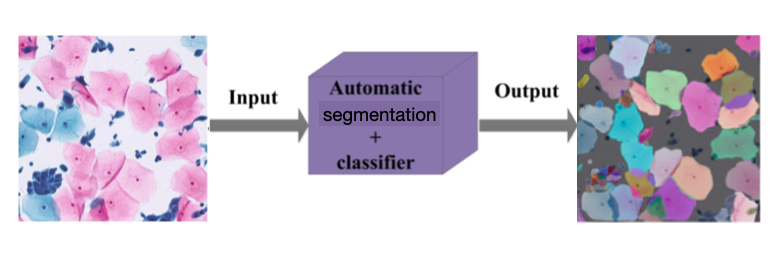
\includegraphics[width=0.5\paperwidth]{TCT/分割样例.png}
    \caption{分割样例图片,左图为样例图片,右图为样例图片的分割结果}
    \label{pic:分割样例}
\end{figure}

\subsection{病变细胞分类与分割}
\par 在临床实践中,医生主要依据细胞核与细胞质的比例,细胞核的大小,细胞核的形状以及核膜的异常变化来判定病变的宫颈细胞,以及区分它们的种类。因此,有许多研究\cite{zhang2014segmentation}\cite{zhang2017graph}\cite{lee2016segmentation}通过分割细胞或细胞的某些部分(细胞核、细胞质),并依据临床上的判定规则完成病变细胞的分类任务。但是由于不同种类细胞的形态差异较大、细胞之间的重叠问题可能比较严重以及细胞质边界可能不够清晰等问题,细胞以及细胞成分的分割依然是一个尚未被很好解决的问题。因此,这类方法往往不能让人满意。
\par 而在另一方面,也有许多研究\cite{marinakis2009pap}\cite{phoulady2016automatic}通过手工设计大量的特征试图捕捉细胞核和细胞质的形态特征,再将这些特征经过特征选择或者降维处理之后输入到各种分类器中(如,随机森林、SVM、神经网络等)来完成分类任务。但是,上述的手工设计的特征往往依赖于细胞或细胞组成成分的分割结果,而且这些手工设计的特征完全来自于当前医学对于宫颈细胞学的认知,因此,此类方法的发展会受到医学发展的限制。

\subsection{病变细胞检测}
\par 近期,病变细胞检测方向的研究主要是基于卷积神经网络进行的。有许多自然图像领域的目标检测模型可以直接用于检测宫颈病变细胞,也有许多研究和工作专门对宫颈病变细胞检测任务提出了做出针对性优化的方法。
\subsubsection{自然图像上的目标检测模型}
\par 绝大多数的目标检测都可以直接用于宫颈病变细胞的检测,他们主要分为One Stage和Two Stage两类。
\paragraph{One stage模型}
\par One stage的典型方法有Joseph\cite{Joseph2018YOLOv3}等提出的YOLOV3,通过将图像分为多个网格之后每个网格预测数个预测框的方式去掉了R-CNN系列在检测过程中所必要的先验框,使模型可以成为One stage的形式。Lin\cite{lin2018focal}等提出的Focal Loss和Retinanet可以大幅削弱类别不平衡对One Stage检测模型的影响,从而使One stage模型可以获得更高的检测性能。Yang\cite{yang2019reppoints}等提出的RepPoints使用点集来表示目标,可以让模型更好的捕获物体的形态特征,进而使模型更好的学习目标潜在的特征信息,从而获得更好的检测性能。Sun\cite{sun2021sparse}等提出的Sparse R-CNN抛弃了Faster R-CNN的RPN结构,使用一个可学习的参数来为后续的检测过程提供目标区域提案,这一方法使得R-CNN系列可以成为End-to-End的模型。
\paragraph{Two Stage模型}
\par 著名的R-CNN系列就是Two Stage的模型,如Ren\cite{ren2015faster}等提出的Faster R-CNN先通过Backbone和FPN提取特征,之后RPN提取目标区域提案,之后使用ROI层提取目标区域提案的特征,并将这些特征送入检测头用于目标检测任务。因此,Faster R-CNN也可以用于宫颈病变细胞的检测。Cai\cite{cai2017cascade}等提出的Cascade R-CNN通过级联多个Faster R-CNN的检测头,将前一阶段的检测头的预测结果当作目标区域提案送入下一阶段的检测头中,通过多阶段不断的优化以获得更好的检测性能。
\subsubsection{宫颈病变细胞检测模型}
\par 也有许多针对宫颈病变细胞检测任务做出专门优化的工作。例如,Ma等\cite{ma2020macd}中设计了新的MACD R-CNN网络,通过在Mask R-CNN的不同分类分支中使用不同的roi提取出一个细胞核特征变形的特征图,将这种特征图与固定roi的特征通过注意力机制合并,最后通过加入更深的卷积层深度提高了检测的精度;Xiang等\cite{xiang2020novel}基于YOLOv3级联了一个额外的特定任务分类器,还通过平滑噪声标签的分布来处理可能存在的不可靠标注,最终提高了宫颈细胞水平诊断的平均精度;Li等\cite{li2019detection}提出了一种基于多语义标签和形态信息分析相结合的目标检测和分类方法,该方法以ResNet101作为骨干网络时可以在LBC数据集上取得66.98\%的平均精度;Liu等\cite{liu2018multitask}使用VGG16迁移学习,并用一种面向任务的基于先验框的网络将产生潜在的感兴趣区域,最后使用全卷积网络来估计细胞的位置并将其分类,这种方法在保持性能和计算效率之间取得了良好的平衡,相较于YOLO和Faster R-CNN它拥有更好的精度和更快的速度,例如,这种方法的耗时只有Faster R-CNN的一半。Liang\cite{liang2018comparison}等提出了基于比较的检测器模型,这个模型在每次迭代的过程中,会首先从选定的参照样本中随机选择固定数量的每一类别的样本,然后与输入图片一同经过Backbone和FPN等结构提取特征,之后将不同类别的样本的特征直接求平均,FPN所得到的不同尺寸的特征也经过一个全局池化层池化为统一大小之后直接求平均,作为该类别的特征。再将所有类别的是特征拼接起来通过一个卷积层得到背景类别的特征。最后将RPN提出的目标区域提案经过ROI层提特征之后,与所有类别的特征计算一个距离,这个距离将被用作分类依据以及回归时的特征,目标区域提案会直接被分到与类别特征最相近的类别,计算出来的距离向量经过两个卷积层和一个全连接层之后也会被当作回归结果用于进一步优化目标区域提案。Liu\cite{liu2018multitask}等提出的多任务模型主要依据Faster R-CNN模型改用了VGG16作为Backbone,并使用了针对宫颈病变细胞数据集专门优化的先验框设置。
\par 目前病变细胞检测方面相关的论文、其所使用的方法、数据集以及最终效果(部分)如\ref{tab:检测论文}:
\begin{table}[htbp]
    \center
    \caption{病变细胞检测论文汇总}
    \begin{tabular}{|p{4cm}|p{4cm}|p{3cm}|p{1cm}|}
        \hline
        论文                                                             & 模型                    & 数据                       & 效果(mAP) \\     \hline
        Faster R-CNN\cite{ren2015faster}                                 & Faster R-CNN            & -                          & -           \\ \hline
        Cascade R-CNN\cite{cai2017cascade}                               & Cascade R-CNN           & -                          & -           \\ \hline
        Sparse R-CNN\cite{sun2021sparse}                                 & Sparse R-CNN            & -                          & -           \\ \hline
        YoloV3\cite{Joseph2018YOLOv3}                                    & YoloV3                  & -                          & -           \\ \hline
        RetinaNet\cite{lin2018focal}                                     & RetinaNet               & -                          & -           \\ \hline
        RepPoints\cite{yang2019reppoints}                                & RepPoints               & -                          & -           \\ \hline
        MACD R-CNN\cite{ma2020macd}                                      & 基于mask R-CNN          & Herlev 数据集              & -           \\ \hline
        Automation-Assisted Reading Method\cite{xiang2020novel}          & YOLO V3 和额外的分类器  & 私有数据12909 例,10个类别 & 0.634       \\ \hline
        Detection in the Limited Data Scenario\cite{liang2018comparison} & Faster R-CNN + FPN      & 私有数据7086例,11个类别   & 0.263       \\ \hline
        Detection and Classification of Cells\cite{li2019detection}      & Faster R-CNN            & 680例,6个类别             & -           \\ \hline
        Multitask Learning for Recognition\cite{liu2018multitask}        & VGG16                   & 73 例                      & -           \\ \hline
        DCCL\cite{zhang2019dccl}                                         & Faster R-CNN,RetinaNet & DCCL公开数据               & -           \\ \hline
    \end{tabular}
    \label{tab:检测论文}
\end{table}
